\chapter{隐藏状态估计：观测算子、可辨识性与滤波}
\label{ch:est}

本章要判定的量是：被动观测对内部热阻的信息在什么条件下为零，以及在线估计器输出的是一个温度点还是决策状态的后验。规格中的估计器是分层的集合滤波。本次日志里的估计器是一个标量跟踪器。二者必须分开写。

\section{可安装观测}

\paragraph{要判定的量}
哪一些通道允许进入品质滤波，哪一些只进入安全约束。

\paragraph{继承的文献层与不继承的层}
观测算子的病态性继承 \cite{ozisik2000}。红外亮度里的发射与反射必须分开，否则加热管的辐射会被当成食品表面温度。不继承某一热像器件的样本噪声作为系统精度。

\begin{table}[ht]
\centering
\caption{进入品质估计器的观测}
\begin{tabularx}{\textwidth}{llX}
\toprule
通道 & 符号 & 与隐藏状态的关系 \\
\midrule
腔体空气温度 & \(y_T\) & 靠近 \(T_\infty\)，受加热器辐射污染 \\
腔体相对湿度 & \(y_\varphi\) & \(p_v/p_{\mathrm{sat}}(T_\infty)\)，饱和时丢失分辨率 \\
食品质量 & \(y_m\) & 累计蒸发的积分，不定位冷点 \\
表面热像 & \(\vect{y}_{\mathrm{IR}}\) & 发射率未知的辐射亮度 \\
电功率 & \(y_P\) & 已知输入，写入边界，不当作食品状态 \\
排气温度 & \(y_{T,e}\) & 冷凝与漏汽的积分证据 \\
\bottomrule
\end{tabularx}
\end{table}

\begin{definition}[观测方程]
\begin{equation}
\label{eq:obs}
\vect{y}_k=h\big(\Phi(\vect{X}(t_k)),\vect{\theta}\big)+\vect{v}_k.
\end{equation}
红外通道
\begin{equation}
\label{eq:ir}
L_j=\epsilon(\varepsilon_{l,s},S_s)\,\sigma T(\vect{r}_j)^4
+\big(1-\epsilon(\varepsilon_{l,s},S_s)\big)L_j^{\mathrm{refl}}.
\end{equation}
\end{definition}

发射率随表面变干下降。系统精度取发射率区间两端分别滤波后的分位包络，不取器件标称精度。协议是四步。发射率取声明区间的两个端点。同一条观测序列在每个端点上各滤波一次。每次滤波给出决策状态的分位区间。系统精度取这两个区间的并集。区间的端点不在本次仓库里，所以包络的宽度没有一个数。

本次核没有热像，也没有质量。进入跟踪器的是表面温度加 \(0.4^\circ\mathrm{C}\) 的确定性散列，以及平均含水加 \(0.004\) 的散列。噪声不是高斯抽样，重复运行得到同一轨迹。上面四步没有被调用。

\paragraph{本节不能推出的结论}
表中的通道是规格。没有采样的通道，不能在结果里出现“去掉该通道后误差上升”这一句。

\section{逆问题的病态结构}

\paragraph{要判定的量}
只加密表面像素，能否稳定恢复冷点。

\paragraph{继承的文献层与不继承的层}
线性化热方程在厚度方向上，对高频边界噪声的放大随 \(\mathrm{e}^{kL}\) 增长 \cite{ozisik2000}。不继承某一个正则化参数作为物理常数。

由此得到四条限制。只加密表面红外像素，不能稳定恢复冷点。必须有一个穿透时间尺度上的动态激励，或一个对内部热阻敏感的积分量。质量损失对累计蒸发敏感，对冷点位置不敏感。先验把解限制在决策流形附近，正则化来自物理，而不是一个随意的光滑惩罚。

\subsection{半无限体上一个谐波的放大}

把“高频边界噪声按 \(\mathrm{e}^{kL}\) 放大”写成一条可核算的振幅比。扩散率取核里的 \(\alpha=2.0\times 10^{-7}\,\mathrm{m}^2/\mathrm{s}\)。坐标 \(x\) 从表面指向食品内部。表面温度取成角频率 \(\omega\) 的谐波，内部满足常系数扩散方程 \(\partial_t T=\alpha\partial_{xx}T\)。试解 \(\mathrm{e}^{\mathrm{i}\omega t}\mathrm{e}^{-sx}\) 代入之后，\(s^2=\mathrm{i}\omega/\alpha\)。实部取正的根用 \(\sqrt{\mathrm{i}}=(1+\mathrm{i})/\sqrt{2}\)，于是
\begin{equation}
\label{eq:halfspace}
T(x,t)=\mathrm{e}^{-kx}\cos(\omega t-kx),
\qquad
k=\sqrt{\frac{\omega}{2\alpha}}.
\end{equation}
深度 \(L\) 处的振幅是表面振幅的 \(\mathrm{e}^{-kL}\)。要从表面记录恢复这个深度上同一频率的振幅，测量噪声乘上 \(\mathrm{e}^{kL}\)。

这一节的几何是半无限体，表面温度是给定的谐波。第 \ref{ch:physics} 章的本征根属于有限厚度平板，一侧绝热，一侧是 Biot 边界。十六条控制体的边界是通量。三套边界各自成立。下表只对 \eqref{eq:halfspace}。

周期取正文里已经出现的时间尺度：演示记录间隔 8 s，战役记录间隔 10 s，探针窗 40 s，满功率加热器时间常数 43.48 s，以及开环三档菜单时间 900 s、1170 s、1530 s。表中把每个时间尺度当成一个谐波的周期，用来回答“若边界里只有这个尺度，深度 \(L\) 处还剩下多少振幅”。核的边界通量并不是这些周期的谐波。

\begin{table}[ht]
\centering
\caption{半无限体上单个谐波的放大倍数 \(\mathrm{e}^{kL}\)。\(\alpha=2.0\times 10^{-7}\,\mathrm{m}^2/\mathrm{s}\)。放大倍数大于 1 表示从表面恢复该深度的同频振幅时，噪声被乘上的因子。}
\small
\begin{tabular}{llrr}
\toprule
周期 & 该尺度在正文中的位置 & \(L\) & \(kL\)，放大 \\
\midrule
8 s & 演示记录间隔 & 15 mm & 21.019，\(1.344\times 10^{9}\) \\
8 s & 演示记录间隔 & 30 mm & 42.037，\(1.806\times 10^{18}\) \\
8 s & 演示记录间隔 & 50 mm & 70.062，\(2.677\times 10^{30}\) \\
10 s & 战役记录间隔 & 15 mm & 18.800，\(1.461\times 10^{8}\) \\
10 s & 战役记录间隔 & 30 mm & 37.599，\(2.134\times 10^{16}\) \\
10 s & 战役记录间隔 & 50 mm & 62.666，\(1.642\times 10^{27}\) \\
40 s & 探针窗 & 15 mm & 9.400，\(1.209\times 10^{4}\) \\
40 s & 探针窗 & 30 mm & 18.800，\(1.461\times 10^{8}\) \\
40 s & 探针窗 & 50 mm & 31.333，\(4.052\times 10^{13}\) \\
43.48 s & 满功率加热器时间常数 & 15 mm & 9.016，\(8.232\times 10^{3}\) \\
43.48 s & 满功率加热器时间常数 & 30 mm & 18.032，\(6.777\times 10^{7}\) \\
43.48 s & 满功率加热器时间常数 & 50 mm & 30.053，\(1.127\times 10^{13}\) \\
900 s & 15 mm 开环菜单 & 15 mm & 1.982，7.255 \\
900 s & 15 mm 开环菜单 & 30 mm & 3.963，52.63 \\
900 s & 15 mm 开环菜单 & 50 mm & 6.606，739.2 \\
1170 s & 30 mm 开环菜单 & 15 mm & 1.738，5.686 \\
1170 s & 30 mm 开环菜单 & 30 mm & 3.476，32.33 \\
1170 s & 30 mm 开环菜单 & 50 mm & 5.793，328.1 \\
1530 s & 50 mm 开环菜单 & 15 mm & 1.520，4.572 \\
1530 s & 50 mm 开环菜单 & 30 mm & 3.040，20.90 \\
1530 s & 50 mm 开环菜单 & 50 mm & 5.066，158.6 \\
\bottomrule
\end{tabular}
\end{table}

8 s 的波数 \(k=1401\,\mathrm{m}^{-1}\)，穿透深度 \(1/k=0.714\,\mathrm{mm}\)。10 s 为 \(0.798\,\mathrm{mm}\)，40 s 为 \(1.60\,\mathrm{mm}\)，43.48 s 为 \(1.66\,\mathrm{mm}\)。菜单时间三档的穿透深度是 7.57 mm、8.63 mm、9.87 mm，都短于对应厚度上的冷点深度。表面 1 K 的 8 s 谐波在 15 mm 处剩下 \(7.44\times 10^{-10}\,\mathrm{K}\)。40 s 谐波在 30 mm 处剩下 \(6.85\times 10^{-9}\,\mathrm{K}\)。家用温度计读不到这个深度上的同频分量。

开环菜单时间把放大降到另一个量级。900 s 谐波在 15 mm、30 mm、50 mm 处的剩余振幅是 0.138、0.0190、\(1.35\times 10^{-3}\)。1170 s 是 0.176、0.0309、\(3.05\times 10^{-3}\)。1530 s 是 0.219、0.0478、\(6.31\times 10^{-3}\)。薄件在自己的菜单时间上还留着约十分之一以上，厚件只留到千分之几。记录覆盖整个菜单，仍然恢复不了厚件冷点上的这个谐波。

令 \(kL=1\)，剩余振幅降到 \(1/\mathrm{e}\)。对应周期是 \(\pi L^2/\alpha\)：15 mm 为 3534 s，30 mm 为 14137 s，50 mm 为 39270 s。三档都长于各自的菜单时间。菜单终点上，半无限体里的冷点深度仍在这个衰减区之内。

\begin{proposition}[静态观测不足以分离内外热阻]
在 \eqref{eq:twonode} 中令三个导数为零且无相变。则 \(T_1=T_2=T_\infty\)，\(R_{\mathrm{int}}\)、\(C_1\)、\(C_2\) 全部从代数方程中消失。
\end{proposition}

完整证明在命题 \ref{prop:steady}。断言在 \(R\in\{1,3,6\}\)、\(T_\infty=100\) 上积分到平衡，温差极差为 0。这是“到时按菜单停机”失败的数学形式：菜单在稳态配方上标定，这一次的内部热阻从未被观察。

\subsection{可观测矩阵的行列式}

沿用 \eqref{eq:fv-obsv} 的两节点线性化。输出只取表面温度，
\[
\mathcal{O}=\begin{pmatrix}\vect{C}\\ \vect{C}\vect{A}\end{pmatrix}
=\begin{pmatrix}1&0\\ -a-b& b\end{pmatrix}.
\]
\[
\det\mathcal{O}=b=\frac{1}{C_1 R_{\mathrm{int}}}.
\]
\(C_1>0\) 且 \(R_{\mathrm{int}}\) 有限时，行列式不为零，两个温度状态可观测。\(R_{\mathrm{int}}\to\infty\) 时行列式趋于零，表面温度不再携带内部节点的信息。厚件在菜单终点的 Fourier 数远小于 1，对应的就是这个方向：不是秩突然消失，而是短时间内灵敏度很小。

平衡点上的参数灵敏度是另一件事。命题 \ref{prop:steady} 已经说明三个温度对 \(R_{\mathrm{int}}\) 的导数为零。把零列放进 \eqref{eq:fisher}，该项贡献是零。因此“状态可观测”不能写成“内部热阻已经可辨识”。探针的作用是离开平衡，让灵敏度列不再是零。

已实现的跟踪器没有组装 \(\mathcal{O}\)，也没有组装 Fisher 矩阵。它用一个标量时间常数跟随表面，再用 \(\hat r\) 把估计压低。方差只在 190 s 之后、而且新的 \(\hat r\) 更接近真值温差参照时，乘一次 0.35。这个参照用了表面与冷点的真值差，所以方差下降不是 \eqref{eq:fisher} 的特征值。

\paragraph{本节不能推出的结论}
病态性不意味着估计不可能。它意味着估计依赖激励和先验。没有激励时增加采样频率无效。\(\mathrm{e}^{kL}\) 是半无限体上单个谐波的振幅比。它不给出十六条控制体的反演误差，也不给出 S1 的残差。

\section{动态可辨识性}

\paragraph{要判定的量}
相变项是否给输入矩阵增加一个与 \(T_\infty\) 线性无关的方向。对 \eqref{eq:twonode}，两列都只进入表面节点，方向共线；要分开的是 \(R_{\mathrm{ext}}\) 与 \(R_{\mathrm{int}}\) 的灵敏度列。

\paragraph{继承的文献层与不继承的层}
灵敏度方程和 Fisher 信息是局部可辨识性的标准构造。不继承本次已经算出了 Fisher 矩阵的特征值。该矩阵没有在日志里计算。

把 \eqref{eq:twonode} 在无相变工作点线性化，状态 \((\delta T_1,\delta T_2)\)，输入 \((\delta T_\infty,\delta v)\)。风速只进入 \(R_{\mathrm{ext}}\)。对输出 \(y=T_1\)，可观测矩阵的秩为 2，内部状态在结构上可观测，但 Gram 矩阵的条件数随 \(R_{\mathrm{int}}/R_{\mathrm{ext}}\) 增大而变坏。厚、干、结壳的食品，表面温度对冷点的响应又慢又弱。

相变项与腔温都写在表面节点的能量平衡上，输入列共线。短蒸汽脉冲仍然改变表面通量的大小，并且不经过 \(R_{\mathrm{ext}}\) 这个系数。参数灵敏度满足
\begin{equation}
\label{eq:sens}
\frac{\mathrm{d}}{\mathrm{d}t}\frac{\partial \vect{s}}{\partial\theta_i}
=\vect{A}(\vect{\theta})\frac{\partial \vect{s}}{\partial\theta_i}
+\frac{\partial \vect{A}}{\partial\theta_i}\vect{s}
+\frac{\partial \vect{B}}{\partial\theta_i}\vect{u},
\end{equation}
其中 \(\vect{s}=(T_1,T_2,m)\)。Fisher 信息
\begin{equation}
\label{eq:fisher}
\vect{\mathcal{I}}(\vect{\theta};\vect{u}_{0:K})
=\sum_{k=0}^{K}
\Big(\frac{\partial h}{\partial \vect{s}}\frac{\partial \vect{s}_k}{\partial\vect{\theta}}\Big)^{\!\top}
\vect{R}_k^{-1}
\Big(\frac{\partial h}{\partial \vect{s}}\frac{\partial \vect{s}_k}{\partial\vect{\theta}}\Big).
\end{equation}
探针设计在规格上最大化 \(\log\det\vect{\mathcal{I}}\) 的增量。断言没有组装这个矩阵。它只比较了两段脉冲与单独蒸汽的表面—内部滞后：\(40.846\) 与 \(38.912\)，判据是差值大于 1。差值大于 1 说明第二段改变了滞后，不说明 Fisher 矩阵的最小特征值已经上升。

\subsection{同一组说明常数上的特征根与有限时域 Gram}

沿用 \eqref{eq:sigma} 的说明常数：\(C_1=C_2=2000\,\mathrm{J/K}\)，\(R_{\mathrm{ext}}=0.05\,\mathrm{K/W}\)，\(R_{\mathrm{int}}=0.15\,\mathrm{K/W}\)。三个系数是
\[
a=\frac{1}{100}\,\mathrm{s}^{-1},\qquad
b=c=\frac{1}{300}\,\mathrm{s}^{-1}.
\]
\(\det(sI-\vect{A})=(s+a+b)(s+c)-bc\)，展开后
\begin{equation}
\label{eq:charpoly}
s^2+\frac{1}{60}s+\frac{1}{30000}=0.
\end{equation}
两个根是 \(-0.014343\,\mathrm{s}^{-1}\) 与 \(-0.002324\,\mathrm{s}^{-1}\)。对应时间常数 \(69.72\,\mathrm{s}\) 与 \(430.3\,\mathrm{s}\)。40 s 的探针窗短于这两个时间常数。慢模态在窗内几乎停在初值附近，所以表面记录在代数上满秩，数值上仍然弱。

腔温输入的列是 \(\vect{B}_T=(a,\,0)^{\mathsf T}\)。可控性矩阵 \([\vect{B}_T,\,\vect{A}\vect{B}_T]\) 的行列式等于 \(a^2 c\)：
\begin{equation}
\label{eq:ctrb}
\det[\vect{B}_T,\,\vect{A}\vect{B}_T]
=\frac{1}{3\,000\,000}\,\mathrm{s}^{-3}.
\end{equation}
\(a\) 与 \(c\) 都为正，所以这一对 \((\vect{A},\vect{B}_T)\) 可控。可控是状态的性质。它不给出 \(R_{\mathrm{int}}\) 的灵敏度。

潜热输入 \(\vect{B}_q=(1/C_1,\,0)^{\mathsf T}\)。它的第一分量与 \(\vect{B}_T\) 的第一分量之比等于 \(R_{\mathrm{ext}}=0.05\,\mathrm{K/W}\)，第二分量都是 0。两列落在同一条直线上。\(q_{\mathrm{lat}}\) 变号只改变这条直线上的倍数，输入矩阵的秩保持为 1。这一核对与命题 \ref{prop:pulse} 的前半句是同一件事，常数就是 \eqref{eq:sigma} 那一组。

有限时域观测 Gram 取输出 \(y=T_1\)，
\begin{equation}
\label{eq:gram}
\vect{W}(T)=\int_0^{T}\vect{\Phi}(t)^{\mathsf T}\vect{C}^{\mathsf T}\vect{C}\,\vect{\Phi}(t)\,\mathrm{d}t,
\qquad
\vect{\Phi}(t)=\mathrm{e}^{\vect{A}t}.
\end{equation}
积分用 4000 步左矩形，转移矩阵用矩阵指数逐步推进，没有闭式。特征值与条件数如下。

\begin{table}[ht]
\centering
\caption{说明常数上的有限时域观测 Gram。条件数是两个特征值之比。它衡量两个温度状态在表面记录里的能量差，不是 \eqref{eq:fisher} 的特征值。}
\begin{tabular}{lrrr}
\toprule
\(T/\mathrm{s}\) & 小特征值 & 大特征值 & 条件数 \\
\midrule
40 & 0.05017 & 24.81 & 494.6 \\
400 & 5.000 & 42.23 & 8.447 \\
1170 & 6.930 & 43.14 & 6.225 \\
\bottomrule
\end{tabular}
\end{table}

40 s 的小特征值是 0.050。窗长到 400 s，已经超过慢时间常数 430 s 的大部分，小特征值升到 5.00，条件数降到 8.45。1170 s 再降到 6.23。探针窗短于慢模态，是这一组常数上 Gram 病态的来源。

固定 \(C_1,C_2,R_{\mathrm{ext}}\)，只改变 \(R_{\mathrm{int}}\)，窗长固定 40 s。条件数随 \(R_{\mathrm{int}}/R_{\mathrm{ext}}\) 增大。

\begin{table}[ht]
\centering
\caption{40 s 窗上，内部热阻与外部热阻之比改变时的 Gram 条件数。热容与 \(R_{\mathrm{ext}}=0.05\,\mathrm{K/W}\) 保持上表。}
\begin{tabular}{rrrr}
\toprule
\(R_{\mathrm{int}}/R_{\mathrm{ext}}\) & 条件数 & 快时间常数 / s & 慢时间常数 / s \\
\midrule
1 & 65.68 & 38.20 & 261.8 \\
3 & 494.6 & 69.72 & 430.3 \\
9 & 4298 & 89.02 & 1011 \\
30 & \(4.735\times 10^{4}\) & 96.67 & 3103 \\
\bottomrule
\end{tabular}
\end{table}

四行都使用同一对热容。比值从 1 增到 30，条件数从 65.7 增到 \(4.74\times 10^{4}\)，慢时间常数从 262 s 增到 3103 s。厚、干、结壳使 \(R_{\mathrm{int}}\) 相对 \(R_{\mathrm{ext}}\) 变大时，40 s 表面记录里内部方向的能量按这个方向变小。Fisher 信息 \eqref{eq:fisher} 没有组装。最小特征值没有一个数字。

\paragraph{本节不能推出的结论}
可观测秩为 2 是线性化结构的结论。它不给出厚件上的估计误差。厚件误差见交叉表，而且那个误差来自标量跟踪器，不是来自 \eqref{eq:fisher} 的实现。特征根、可控性行列式和 Gram 条件数使用 \eqref{eq:sigma} 的说明常数。它们不是 Fisher 信息的特征值，也不是十六条控制体格式的谱。

\section{贝叶斯估计器}

\paragraph{要判定的量}
在线更新的是哪一层参数，控制器读的是均值还是分位数。

\paragraph{继承的文献层与不继承的层}
集合卡尔曼滤波的预测—分析结构继承 \cite{evensen2003}。不继承本次已经用 32 个成员跑完了主表。没有这次运行。

规格分三层。

\begin{enumerate}
\item 参数层。\(\vect{\theta}=(C_1,C_2,R_{\mathrm{int}},R_{\mathrm{ext}},k_m,K_{\mathrm{ev}})\)。先验按类别读取。过程噪声只加在会漂移的项上，例如结壳使 \(R_{\mathrm{int}}\) 随 \(S\) 增大。
\item 场层。一维径向降阶模型的模态系数用集合卡尔曼滤波更新。集合成员共享当前参数后验的抽样。实时集合规模 32，离线对照 128。预测协方差加膨胀因子，空间局部化用 Gaspari--Cohn 函数，半径取一至两个节点。
\item 决策层。每个成员计算 \(\vect{z}^{(i)}=\Phi(\vect{X}^{(i)})\)。控制器使用分位数，不使用集合均值一个数。
\end{enumerate}

湿度通道在读数超过 0.98 时增大对应的观测方差，表示饱和段几乎没有信息。红外似然使用 \eqref{eq:ir}，发射率与表面结壳绑定，作为慢变参数。

\subsection{规格中的分析步}

集合更新按下面的顺序写，供实现时对照。本次积分没有集合成员，所以下面各式没有被调用。

预测步把每个成员按当前参数抽样积分一个离散步，得到预报 \(\vect{x}^{(i),f}\)。记集合均值 \(\bar{\vect{x}}^{f}\) 与异常
\[
\vect{X}'=\big[\vect{x}^{(1),f}-\bar{\vect{x}}^{f},\,\ldots,\,\vect{x}^{(N),f}-\bar{\vect{x}}^{f}\big].
\]
预报协方差取
\begin{equation}
\label{eq:enkf}
\vect{P}^{f}=\frac{\beta}{N-1}\,\vect{X}'(\vect{X}')^{\mathsf T}.
\end{equation}
膨胀因子 \(\beta\ge 1\)。规格没有把它定成一个数。空间上，径向距离超过一至两个节点的相关置零；近处的权在零距离为 1，在截断距离为 0。观测算子在当前均值处线性化为 \(\vect{H}\)。增益
\[
\vect{K}=\vect{P}^{f}\vect{H}^{\mathsf T}
\big(\vect{H}\vect{P}^{f}\vect{H}^{\mathsf T}+\vect{R}\big)^{-1}.
\]
分析步的均值是 \(\bar{\vect{x}}^{a}=\bar{\vect{x}}^{f}+\vect{K}(\vect{y}-\vect{H}\bar{\vect{x}}^{f})\)。成员更新可以走扰动观测，也可以走均方根形式。规格允许两种实现，日志没有选定哪一种。

控制器读的是成员映射到 \(\vect{z}\) 之后的经验分位数。实时集合规模 32、离线对照 128，是规格里的集合大小，不是本次积分的重复次数。湿度读数超过 0.98 时增大 \(\vect{R}\) 的对应对角元。这条规则已经写在观测通道上，分析步不再另给一个阈值。

\paragraph{已运行的跟踪器}
本次没有集合，没有膨胀，没有局部化。状态是三个标量：\(\hat r\) 初值 5，方差初值 0.64，\(\hat T_c\) 以时间常数
\begin{equation}
\tau=\mathrm{clip}(\hat r,0.8,8)\,(L/0.03)^2\cdot 280\ \mathrm{s}
\end{equation}
跟踪表面温度，并被截到表面读数减去 \(4\max(\hat r-1,0.2)\)。对偶策略在 190 s 之后按附录 \ref{app:discrete} 的规则更新 \(\hat r\)，只有更接近真值参照时才把方差乘 0.35。这个参照使用了真值温差，所以分析步不是集合卡尔曼的分析步。

30 mm、\(\hat r=5\) 时 \(\tau=1400\,\mathrm{s}\)。表面温度在几分钟内可以到 \(100^\circ\mathrm{C}\) 以上，估计冷点以约 23 min 的时间常数去追它，同时被滞后上限压住。种子 7 在 1200 s 时估计已经高于冷点，说明上限没有构成下置信界。交叉表里厚件仍然提前停止，与这个跟踪器的结构一致：厚度使 \(\tau\) 按 \(L^2\) 增大，但滞后上限只按 \(\hat r\) 给一个常数，表面远高于冷点之后估计仍可越过阈值。

\paragraph{同一核的成员散布}
另有一份日志，把同一条对偶核重复积分 32 次和 128 次。成员只改种子，种子为 \(1000\) 加成员序号。食品是肉糜，初温 \(8^\circ\mathrm{C}\)，含水 0.72，记录间隔 80 s。没有卡尔曼增益，没有分析步，也没有把成员方差写回下一步。热力进度的成员标准差在全部 12 组里最大为 \(0.0011\)，结束时为 0。停机误差的宽度来自停止时刻，不来自进度轨迹的分叉。

128 个成员、均匀场：15 mm 的 \(e_{50}=-0.1091\)，十分位到九十分位为 \([-0.1104,-0.1073]\)；30 mm 为 \(-0.0954\)，区间 \([-0.0959,-0.0948]\)；50 mm 的三个分位都是 \(-0.7066\)。导热降到 0.45 倍的那一档：15 mm 的中位数 \(-0.4607\)，九十分位到进度上沿 \(+0.150\)；30 mm 为 \(-0.2027\)，区间 \([-0.2034,-0.2019]\)；50 mm 的三个分位都是 \(-0.8024\)。32 个成员的中位数与 128 个相差不超过 \(0.0005\)。终点方差在 12 组里都是 0.224，因为对偶窗把初值 0.64 乘了 0.35，成员没有各自的方差。

\begin{figure}[ht]
\centering
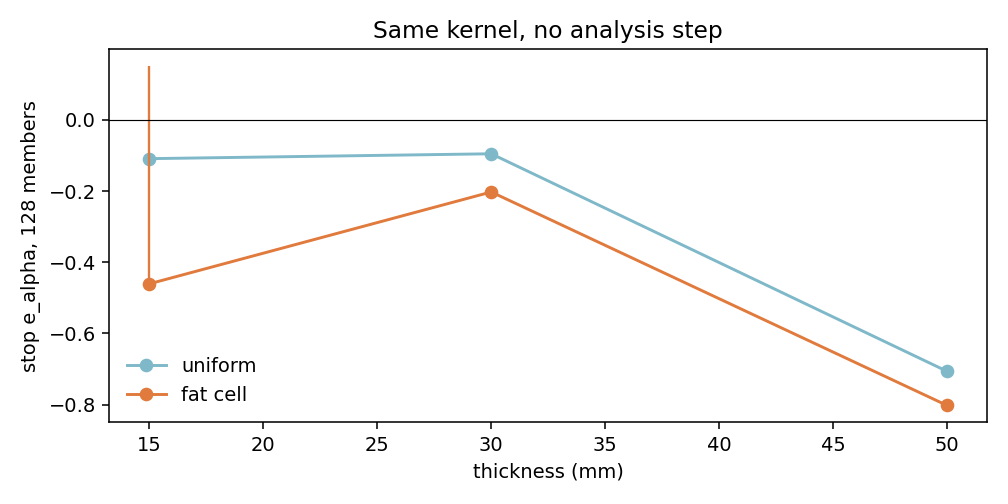
\includegraphics[width=0.86\textwidth]{E_ensemble.png}
\caption{同一对偶核、128 个成员的停机误差。竖线是十分位到九十分位。没有分析步，所以这不是集合滤波的协方差。}
\end{figure}

\paragraph{本节不能推出的结论}
不能把 128 与 32 的中位数之差写成集合规模不足。差不超过 \(0.0005\)，是因为噪声几乎不推动这条对偶轨迹。不能把方差乘 0.35 写成后验熵的奈特数。

\section{可观测性失效时的行为}

\paragraph{要判定的量}
估计器在什么条件下失去输出点预测停机的权利。

三条规格条件：Fisher 矩阵的最小特征值低于类别阈值；质量通道与湿度通道的残差超过三倍标准差并持续一个热时间常数；集合成员的 \(\alpha_m\) 分位区间同时覆盖“未达安全”和“已经过熟”。第三条必须由探针或低功率保温来压缩区间，不能靠把阈值调低来选择一边。

本次核没有特征值，没有质量通道。上面的成员散布是积分之后的统计，没有在积分过程中检查分位区间。退化后的在线行为只有一条：对偶策略在 \(L>40\,\mathrm{mm}\) 且方差仍大于 0.45 时否决停止。否决之后请求可以继续，但停止时刻不因该次探针而提前。50 mm 的成员误差全部落在设计线之下，区间宽度为 0，这条否决没有因为成员变多而改变。

\paragraph{本节不能推出的结论}
失效条件写出来，不等于失效已经被注入并计数。表面保持、质量通道、脂肪层和一次开门在 S2 里有 40 个种子的记录。噪声倍数没有单独扫描。

\section{本章与前后章的接口}

本章的规格产出是 \(p(\vect{z},\vect{\theta}\mid\vect{y}_{0:k})\) 与 Fisher 信息。第 \ref{ch:ati} 章读取它们决定要不要探针。第 \ref{ch:causal} 章读取结构方程的当前参数。第 \ref{ch:safe} 章读取分位数做机会约束。任何下游模块若只接收均值，视作违反第 \ref{ch:arch} 章的合同。

本次实际交出的是 \((\hat T_c,\hat r,\mathrm{Var}(r))\)。下游策略把 \(\hat T_c\) 放进一个饱和线性律。这个接口比合同窄。窄接口上的策略比较仍然可以做，但结论的主语是这个跟踪器，不是集合滤波。
